\documentclass{article}      % Specifies the document class
\usepackage[margin=1in]{geometry}
\usepackage{caption}
\usepackage[final]{graphicx}
\usepackage{amsmath}
\usepackage{placeins}
\usepackage{float}           % Add float package for [H] option
\usepackage[T1]{fontenc}
\usepackage{booktabs}
\usepackage[table]{xcolor}
\usepackage{array}
\usepackage{colortbl}
\usepackage{rotating}
\usepackage{makecell}
\usepackage{url}

\definecolor{lightgray}{gray}{0.7}
\title{Case Study 6: HEPMASS Event Classification with PyTorch-Based Neural Networks}
\author{Kristin Henderson}
\date{July 20, 2025}         % Deleting this command produces today's date.

\newcommand{\ip}[2]{(#1, #2)}
                             % Defines \ip{arg1}{arg2} to mean
                             % (arg1, arg2).
                             
\begin{document}             % End of preamble and beginning of text.

\maketitle                   % Produces the title.

\section{Introduction}       % Produces section heading.  Lower-level
                             % sections are begun with similar
                             % \subsection and \subsubsection commands.

The goal of this study is to use the HEPMASS "all" dataset\footnote{\url{https://archive.ics.uci.edu/dataset/347/hepmass}}, which simulates high-energy particle collisions, to train a neural network binary classifier that distinguishes signal events (class 1, \texttt{particle detected})---those that produce new particles---from background events (class 0, \texttt{no particle}) that do not.

\section{Data}

\subsection{Dataset}

The provided HEPMASS dataset (\texttt{all\_train}) contains 7 million labeled events, evenly split between signal (1) and background (0) classes, as shown in Figure~\ref{fig:target_classes}. Each event includes 27 numerical physics features with varied distributions---normal, skewed, bimodal/discrete, or uniform---and a discrete mass feature taking one of five values: 500, 750, 1000, 1250, or 1500. Representative histograms of several features are shown in Figure~\ref{fig:representative_distributions}. 

\begin{figure}[!htbp]
	\centering
	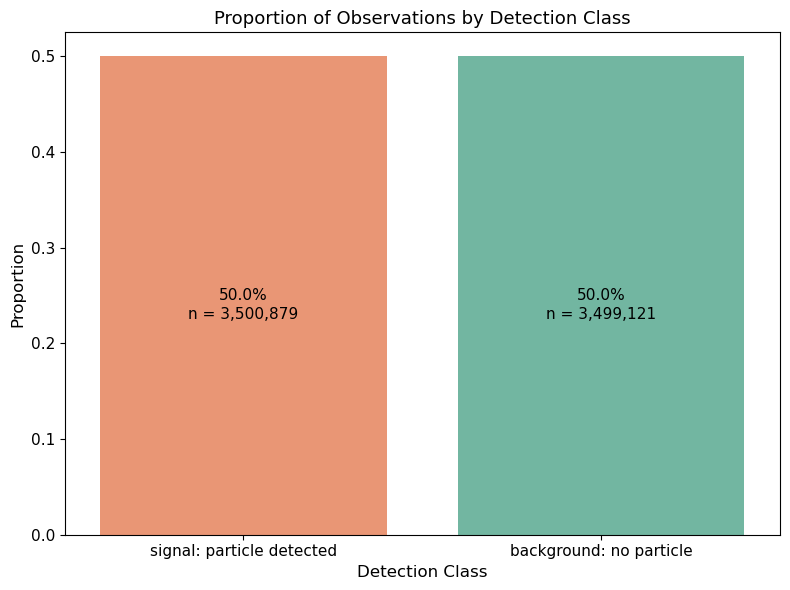
\includegraphics[width=0.60\textwidth]{figures/target_classes.png}
    \caption{Proportion of observations in each event class. Counts and percentages are labeled on the bars.}
	\label{fig:target_classes}
\end{figure}

\begin{figure}[!htbp]
	\centering
	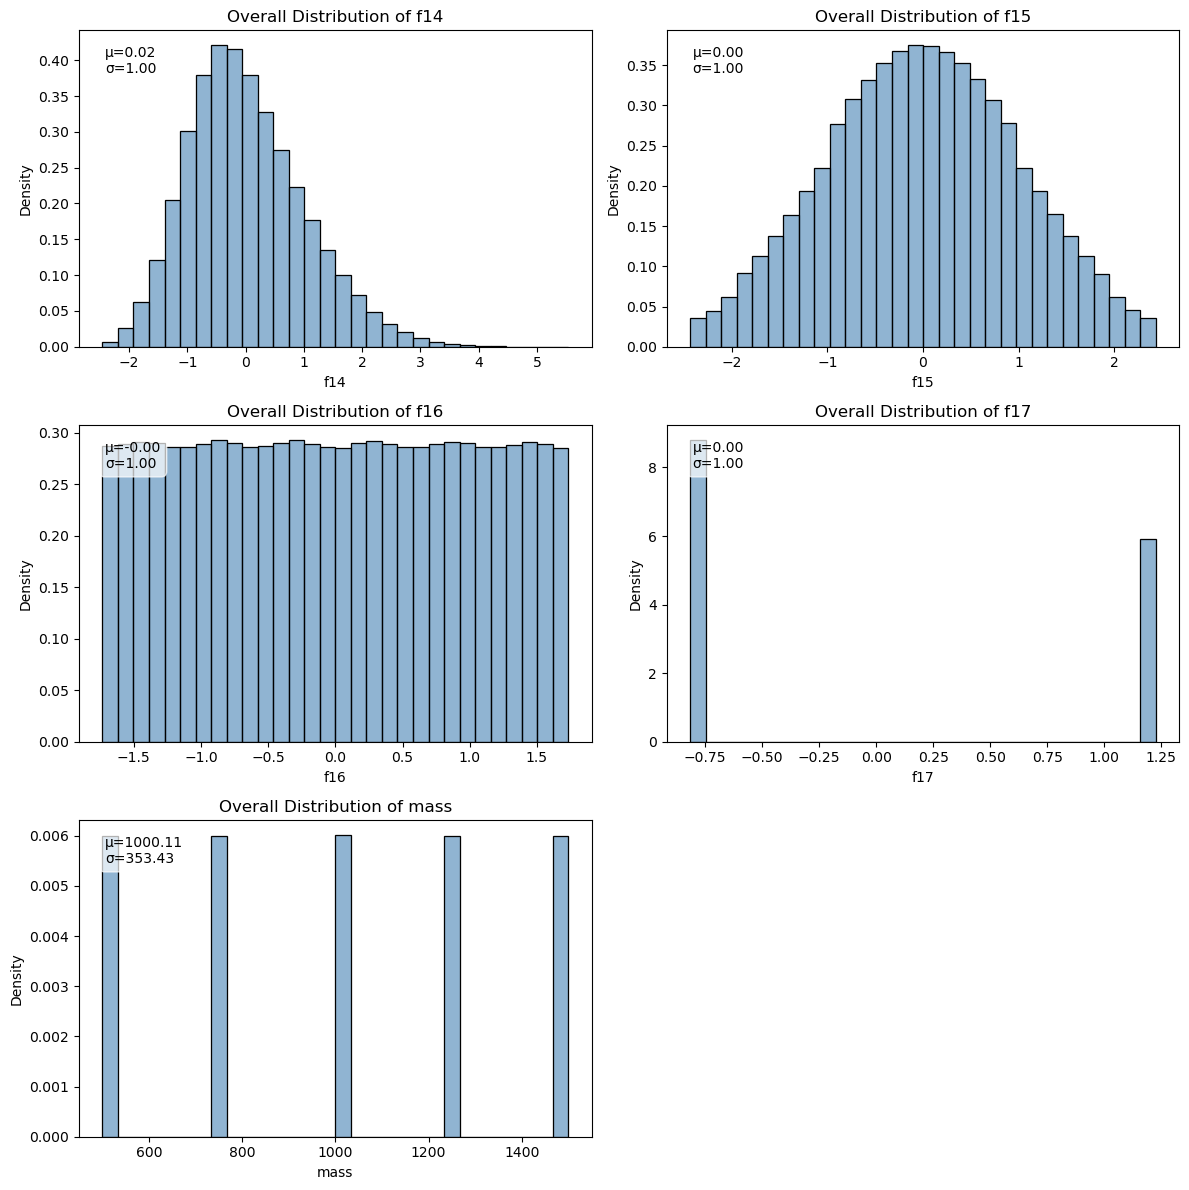
\includegraphics[width=1.0\textwidth]{figures/representative_distributions.png}
    \caption{Representative histograms of the varied distributions of features including mass.}
	\label{fig:representative_distributions}
\end{figure}

For signal events, the mass feature reflects the simulated mass of the new particle. For background events, the value is randomly sampled from the same set to prevent the model from relying on mass alone. All features except for the mass feature appear approximately standardized with mean 0 and standard deviation 1. A summary is provided in Table~\ref{table:features}.

\begin{table}[!htbp]
    \centering
    \caption{HEPMASS Dataset Features}
    \small  % or \footnotesize for even smaller
    \begin{tabular}{lll}
    \arrayrulecolor{black}  % Start with black rules
    \toprule
    \textbf{Feature} & \textbf{Description} & \\
    \midrule
    \arrayrulecolor{lightgray}
    \texttt{f0}, \ldots, \texttt{f26} & Numerical physics features \\ \hline
    \texttt{mass} & Mass: & signal particle (signal events) \\
    & & dummy value (background events) \\ \hline
    \texttt{\# label} & Target class: & \texttt{particle detected} (signal, 1) \\
    & & \texttt{no particle} (background, 0) \\
    \arrayrulecolor{black}
    \bottomrule
    \end{tabular}
    \label{table:features}
\end{table}

\subsection{Preprocessing}

There are no missing values in the dataset. To improve computational efficiency the features were converted from 64-bit to 32-bit floating point values.

Because neural networks are sensitive to feature scales, \texttt{StandardScaler()} was applied to mass---and precautionarily to the remaining features---to ensure stable gradients, sensible weight initialization, and activation values that remain in effective learning ranges. This scaling helps reduce the risk of vanishing gradients and improves overall training efficiency.

The dataset was split into training and validation sets using an 80/20 stratified and shuffled split. Because PyTorch Lightning was being used for modeling, both the training and validation sets were converted to PyTorch tensors.

\section{Modeling}
\subsection{Setup for All Models}

\texttt{DataLoader()} was used to create batches of 1024 samples. For the training set, \texttt{shuffle=True} was applied to randomize the sample order, which promotes better generalization during learning. For validation, \texttt{shuffle=False} was used to ensure consistency across epochs by feeding the model the same validation data in the same order every time.

Early stopping was implemented to prevent overfitting. The \texttt{EarlyStopping()} callback monitored validation accuracy (\texttt{val\_accuracy}), using the default \texttt{min\_delta=0} and \texttt{patience=5}. This means training continued as long as there was any improvement in validation accuracy, but stopped after 5 consecutive epochs without improvement indicating convergence.

CSV logging was used to track loss and accuracy metrics per epoch. Additionally, model checkpoints were automatically saved during training to enable resuming or evaluating models.

\subsection{Base Model}

A baseline model was constructed using a simple feedforward neural network with one hidden layer of 100 neurons. The 28 scaled input features---27 physics variables plus a discrete mass value---were passed through this hidden layer with a Gaussian Error Linear Unit (GELU) activation function. GELU was chosen for its smooth, non-linear behavior and training stability. It belongs to the ReLU family but avoids the “dying ReLU” problem, reduces sudden gradient jumps, and lowers the risk of vanishing gradients. Its robustness allows it to perform well across different datasets and architectures without additional tuning.

The final output layer used a single neuron with a sigmoid activation to produce probabilities for binary classification. The model was trained using the Adam optimizer with a learning rate of 0.001 and binary cross-entropy (BCE) as the loss function.

Adam was selected over a traditional optimizer like Stochastic Gradient Descent (SGD) because it is a modern, adaptive method that combines momentum and per-parameter learning rate adjustment. Momentum helps the optimizer remember the direction of past gradients, smoothing the learning path, and reducing the risk of getting stuck in local minima or noisy updates. Adam is widely recommended as a default choice for deep learning due to its stability and efficiency.

A learning rate of 0.001 was used as a standard baseline, as this value often performs well when paired with the Adam optimizer and offers a good balance between learning speed and convergence reliability.

A summary of all model configurations is provided in Table~\ref{table:model_configurations}.

\subsection{Dense Model}

To test whether greater model complexity could improve performance, a deeper feedforward neural network was built with five hidden layers, each containing 1000 neurons, and GELU activations between layers. The same 28 scaled features served as input, and the output layer again used a sigmoid function to produce probabilities for classification.

This deeper network used the Adam optimizer with a reduced learning rate of 0.0001. A smaller learning rate was necessary because, at higher rates, the predicted probabilities tended to hover around 0.5, suggesting that the model was not effectively learning. Binary cross-entropy was again used as the loss function.

\subsection{Dropout Model}

To explore whether overfitting was limiting performance and whether regularization could help, the Dense model was modified to include dropout layers after each hidden layer. The dropout rate was set to 0.2, meaning that 20\% of the neurons were randomly disabled during training. This helps prevent overfitting by encouraging the network to learn more robust and generalizable features. A rate of 0.2 is a commonly used default that provides effective regularization while preserving sufficient capacity for learning. This Dropout model architecture serves as the foundation for the subsequent Leaky and Swish models, which maintain identical structure but use different activation functions.

Again, the model was trained using the Adam optimizer with a learning rate of 0.0001 and the BCE loss function.

\subsection{Leaky and Swish Models}

Two additional models were built using the same architecture, optimizer, learning rate, and loss function as the Dropout model, but with different activation functions. The first model used a Leaky Rectified Linear Unit (Leaky ReLU) activation function, a variant of Rectified Linear Unit (ReLU) that allows small negative outputs instead of zero. This helps prevent neurons from becoming inactive (“dying”) and is also less computationally intensive than GELU.

The second model used the Sigmoid Linear Unit (SiLU), also known as Swish, a smooth, non-monotonic activation function that allows small negative values and improves gradient flow. Swish often performs well in very deep or wide networks due to its flexibility and smoother transitions compared to other commonly used ReLU-based activations. SiLU is also less computationally intensive than GELU.

\subsection{LRScheduler Model}

To explore whether a more adaptive optimization strategy could improve training, this model used the AdamW optimizer together with an OneCycleLR learning rate scheduler. The architecture, activation functions, and loss function were otherwise the same as in the Swish model. AdamW is a variant of Adam that decouples weight decay from the gradient update, applying regularization directly to the weights instead of through the gradients. This tends to improve generalization, especially in deep networks. The learning rate followed a one-cycle policy: it started low, increased to a peak of 3e-4 during the first 30\% of training, then gradually decreased to a much smaller final value using cosine annealing. Scheduler parameters followed standard defaults: \texttt{div\_factor=25} (initial LR = 3e-4 / 25 = 1.2e-5) controlled the initial learning rate, \texttt{final\_div\_factor=10000} (final LR = 3e-4 / 10000 = 3e-8) set the final learning rate, and \texttt{pct\_start=0.3} defined the warm-up portion. As with previous models, early stopping was used to prevent overfitting. While these choices were exploratory, the goal was to test whether combining adaptive rate control with more direct weight regularization could improve learning efficiency.

\subsection{Training Setup}

Training was conducted on Google Colab using a high-RAM L4 GPU instance. PyTorch Lightning was used for model development and evaluation, with a fixed random seed (set to 13) to support reproducibility. Some inherent randomness remained due to dropout (which randomly disables neurons during training), contributing to slight variability in training duration and the number of epochs required before early stopping. Scikit-learn was used to calculate evaluation metrics. 

Figure~\ref{fig:training_curves} summarizes the training and validation loss and accuracy for all six models over time. Figure~\ref{fig:training_curves_specific} shows the training and validation curves on the same axes for the Swish and Dropout models, which differ only in their activation functions (SiLU vs.\ GELU).

\begin{figure}[!htbp]
    \centering
    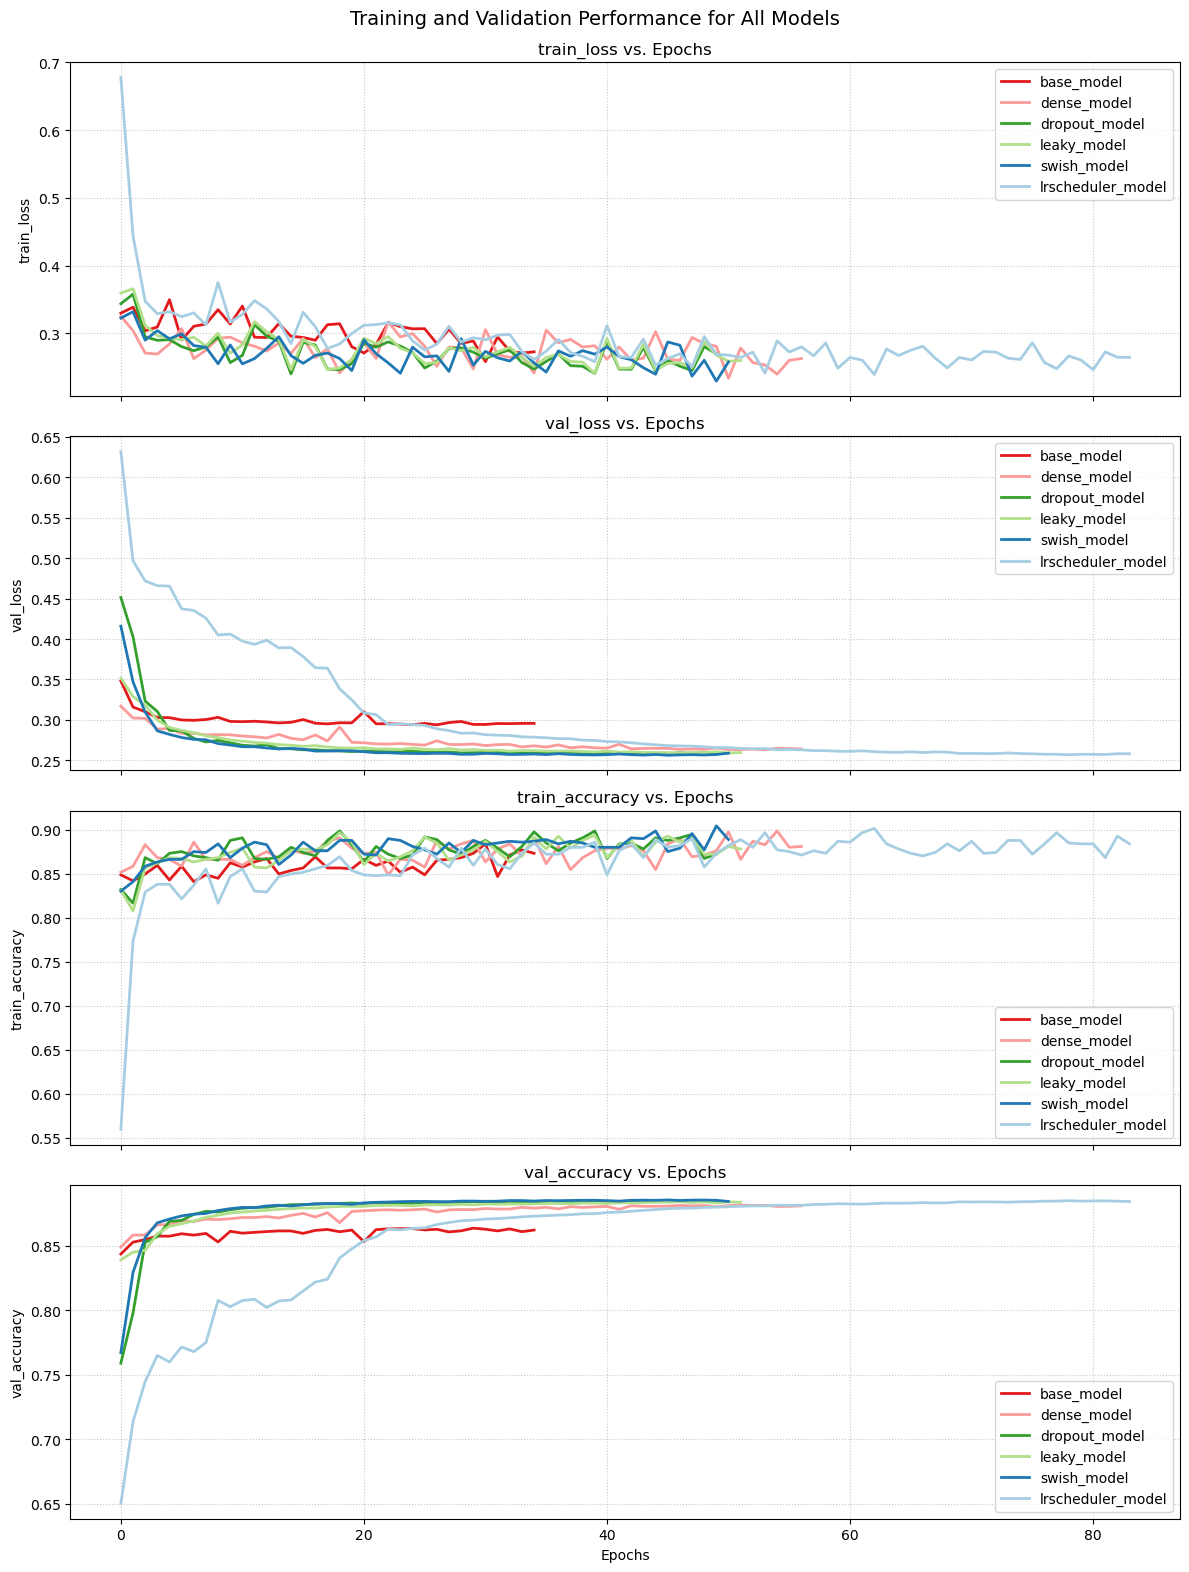
\includegraphics[width=1.0\textwidth]{figures/training_dynamics.png}
    \caption{Training and validation curves for BCE loss and accuracy for all models.}
    \label{fig:training_curves}
\end{figure}

\begin{figure}[!htbp]
    \centering
    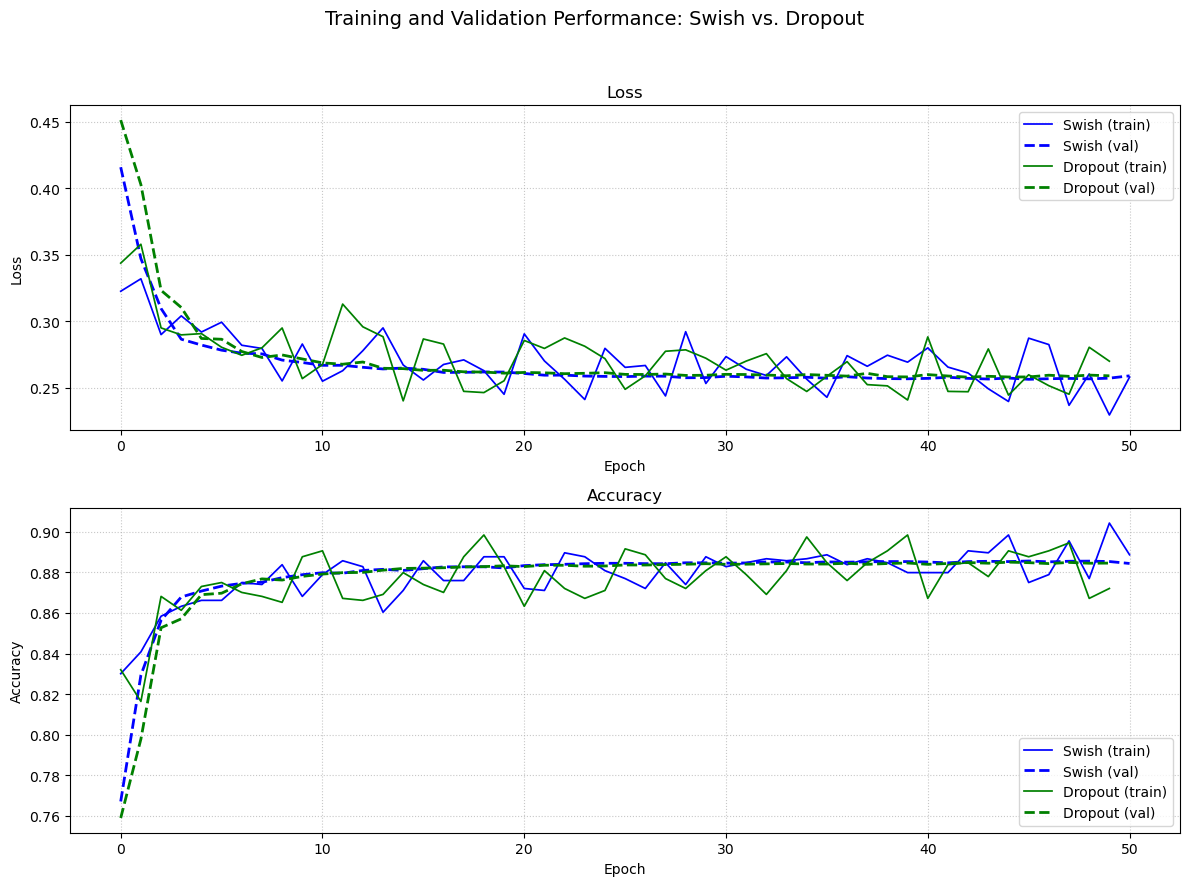
\includegraphics[width=1.0\textwidth]{figures/training_dynamics_specificModels.png}
    \caption{Training and validation curves for BCE loss and accuracy plotted on the same axis for the Swish and Dropout models, which differ only in their activation functions (SiLU vs.\ GELU).}
    \label{fig:training_curves_specific}
\end{figure}

\FloatBarrier
\subsection{Summary of Model Configurations}

\begin{table}[H]
    \centering
    \caption{Neural Network Configuration by Model}
    \begin{tabular}{lcccc}
    \arrayrulecolor{black}
    \toprule
    \textbf{Model} & \textbf{Hidden Layers / Units} & \textbf{Activation} & \textbf{Optimizer} & \textbf{Learning Rate} \\
    \midrule
    \arrayrulecolor{lightgray}
    Base             & 1 x 100      & GELU   & Adam   & Fixed (0.001) \\ \hline
    Dense            & 5 x 1000     & GELU   & Adam   & Fixed (0.0001) \\ \hline
    Dropout          & 5 x 1000     & GELU   & Adam   & Fixed (0.0001) \\ \hline
    Leaky            & 5 x 1000     & LeakyReLU & Adam & Fixed (0.0001) \\ \hline
    Swish            & 5 x 1000     & SiLU   & Adam & Fixed (0.0001) \\ \hline
    LRScheduler      & 5 x 1000     & SiLU   & AdamW & OneCycle (max: 0.0003) \\
    \arrayrulecolor{black}
    \bottomrule
    \end{tabular}
    \vspace{0.5em}
    \caption*{\small\textit{Note: All models were trained using binary cross-entropy loss and a final sigmoid activation for binary classification. Early stopping was applied with a patience of 5 and validation accuracy as the monitored metric. The \texttt{OneCycleLR} learning rate schedule used \texttt{pct\_start = 0.3}, \texttt{div\_factor = 25}, and \texttt{final\_div\_factor = 10000}, increasing to a max of 0.0003 before cosine annealing downward.}}
    \label{table:model_configurations}
\end{table}

\section{Results}

\subsection{Validation Set Results}

\subsubsection{Confusion Matrices}

To generate the confusion matrices shown in Figure~\ref{fig:validation_confusion_matrices}, a default classification threshold of 0.5 was used for all models. This threshold was appropriate because the target classes were balanced, and no explicit priority was placed on detecting one class over the other.

All models demonstrated similar patterns of misclassification, particularly among the five multilayer network architectures. The target classes were nearly balanced. As a result, the misclassifications likely reflect differences in model behavior, such as decision boundary shape and sensitivity, rather than class imbalance.

The Base model consistently underperformed, yielding the lowest number of correct predictions for both classes. It was the only model to correctly classify fewer than 600,000 \texttt{no particle} events and misclassified more than 70,000 \texttt{particle detected} events as \texttt{no particle}. It also produced the highest number of false positives, incorrectly labeling over 100,000 \texttt{no particle} events as \texttt{particle detected}.

Among the remaining five models, the Swish model achieved the highest correct \texttt{no particle} classification count (609,660), narrowly outperforming the Leaky model (606,410), but with a slightly lower \texttt{particle detected} count (628,491). In contrast, the Dense model (without dropout) correctly identified the most \texttt{particle detected} events (638,151), followed closely by the Dropout model (635,478). However, both of these models correctly classified just over 600,000 \texttt{no particle} events, indicating a potential trade-off in optimizing performance between the two classes.

\begin{figure}[!htbp]
	\centering
	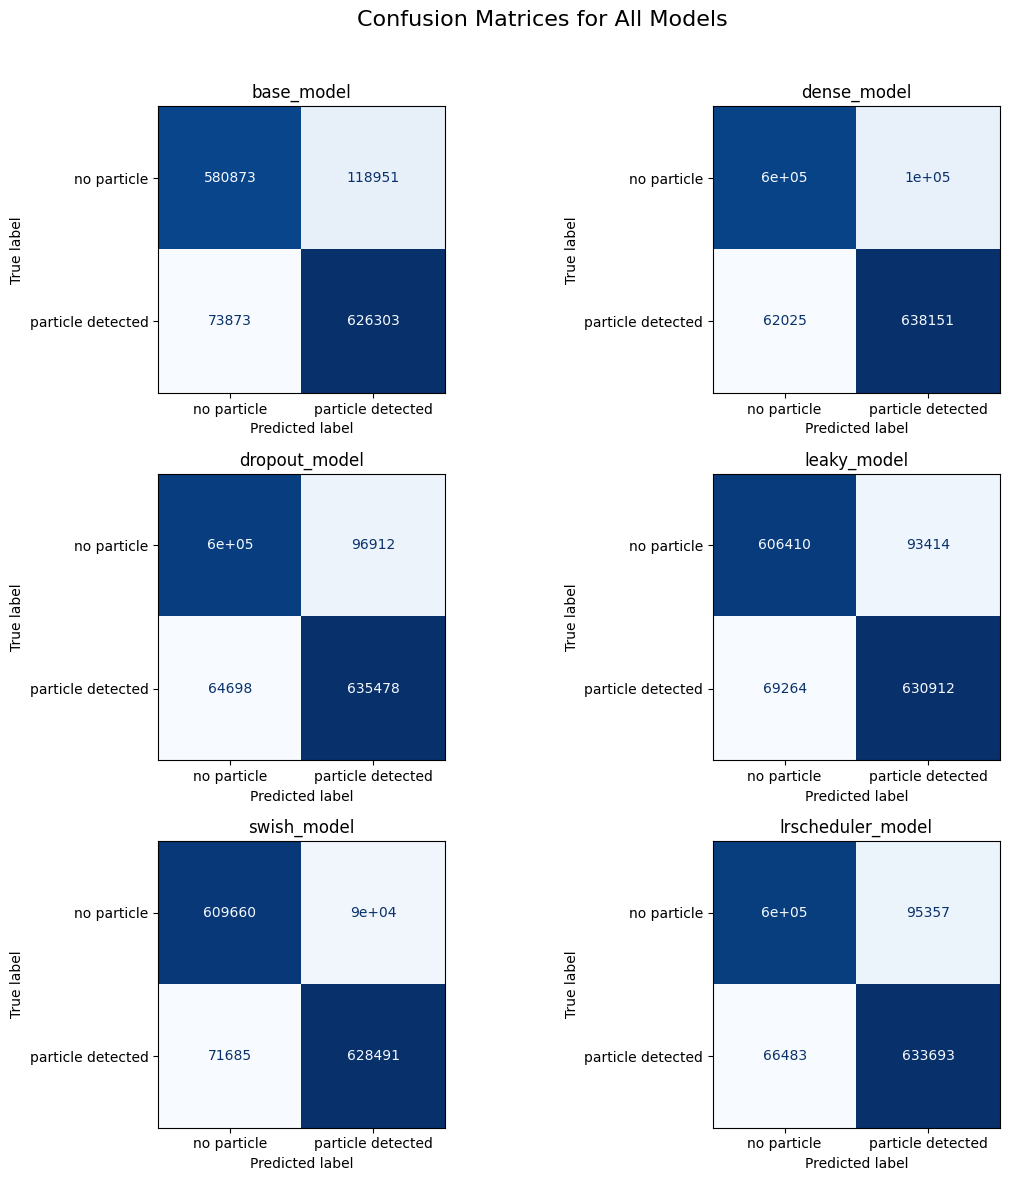
\includegraphics[width=1.0\textwidth]{figures/confusion_matrices_validation.png}
	\caption{Confusion matrices showing classification results from the validation set for all models. True labels are on the vertical axis and predicted labels on the horizontal axis. Each cell indicates the number of instances classified into each category.}
	\label{fig:validation_confusion_matrices}
\end{figure}

\subsubsection{Overall Metrics}

All six models achieved similar overall metrics. Accuracy, macro-averaged precision, recall, and F1-score values ranged from 0.862 to 0.885, as shown in Table~\ref{table:overall_metrics}. The Base model had the lowest scores (accuracy: 0.8623 and similar values for macro-averaged metrics) but the shortest training and prediction times. 

The highest accuracy, 88.46\%, was achieved by the Dropout model, which used GELU activation and the Adam optimizer. The Swish model, which used the SiLU activation function and Adam, achieved 88.44\%. The LRScheduler model, combining SiLU, AdamW, and a OneCycle learning rate schedule, also reached 88.44\%. Training time was just over an hour for the Dropout and Swish models, but nearly two hours for the LRScheduler model, which was by far the longest. These three also had the highest macro-averaged precision, recall, and F1-score.

The Leaky model performed slightly worse than those top three but outperformed the Dense model (which lacked dropout) in both speed and overall metrics.

Since the target classes were balanced, macro and weighted averages were nearly identical. As a result, macro-averaged metrics are reported as a reliable and concise summary. These trends are visually summarized in Figure~\ref{fig:validation_metrics_bar}.

\begin{table}[!htbp]
    \centering
    \caption{Overall Metrics and Training Time by Model on the Validation Set}
    \begin{tabular}{lccccccc}
    \arrayrulecolor{black}
    \toprule
    \textbf{Model} & \textbf{Accuracy} & \textbf{\makecell{Macro\\Precision}} & \textbf{\makecell{Macro\\Recall}} & \textbf{\makecell{Macro\\F1}} & \textbf{Epochs} & \textbf{\makecell{Training\\Time (min)}} & \textbf{\makecell{Prediction\\Time (sec)}} \\
    \midrule
    \arrayrulecolor{lightgray}
    Base & 0.8623 & 0.8638 & 0.8623 & 0.8621 & 34 & 46.50 & 14.64 \\ \hline
    Dense & 0.8811 & 0.8825 & 0.8811 & 0.8810 & 56 & 78.03 & 15.12 \\ \hline
    Dropout & 0.8846 & 0.8854 & 0.8846 & 0.8845 & 49 & 67.41 & 15.02 \\ \hline
    Leaky & 0.8838 & 0.8843 & 0.8838 & 0.8838 & 51 & 72.15 & 14.91 \\ \hline
    Swish & 0.8844 & 0.8847 & 0.8844 & 0.8844 & 50 & 70.54 & 14.92 \\ \hline
    LRScheduler & 0.8844 & 0.8851 & 0.8844 & 0.8843 & 83 & 117.63 & 13.83 \\
    \arrayrulecolor{black}
    \bottomrule
    \end{tabular}
    \caption*{\small\textit{Note: Macro and weighted metrics are nearly identical due to class balance. Only macro-averaged metrics are reported for brevity.}}
    \label{table:overall_metrics}
\end{table}

\begin{figure}[!htbp]
    \centering
    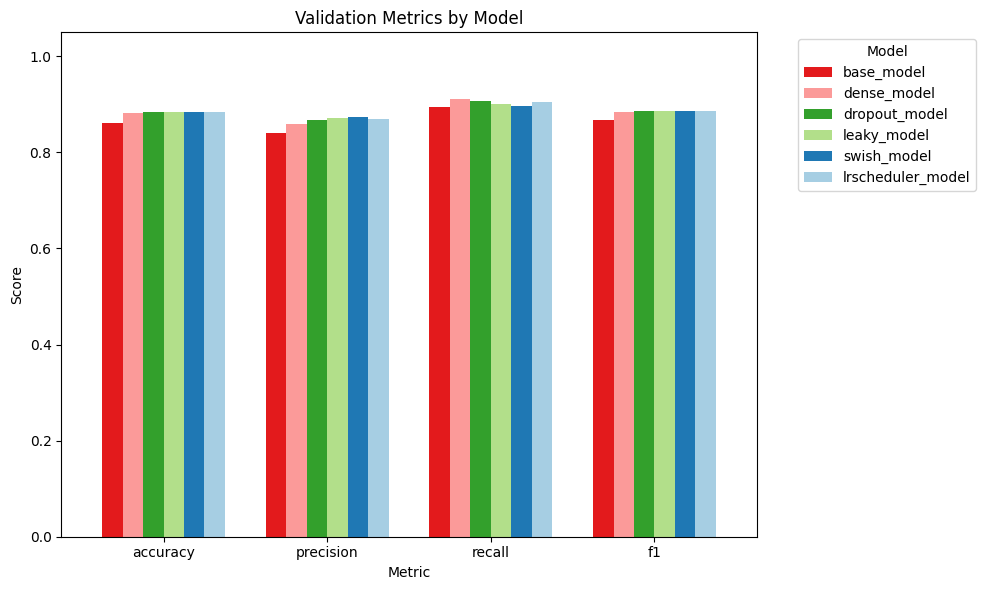
\includegraphics[width=0.80\textwidth]{figures/evaluation_metrics_validation.png}
    \caption{Bar chart of validation set performance metrics (accuracy, precision, recall, F1-score) for each model. Values reflect macro-averaged scores.}
    \label{fig:validation_metrics_bar}
\end{figure}
 
\subsubsection{Per-Class Metrics}

As shown in Table~\ref{table:metrics_by_class}, all models exhibited a consistent trend: higher precision than recall for the \texttt{no particle} class, and higher recall than precision for the \texttt{particle detected} class. The F1-score was higher for the \texttt{particle detected} class across all models.

For the \texttt{no particle} class, the Dense and Dropout models achieved the highest precision (0.9056 and 0.9031, respectively), while the Swish and Leaky models achieved the highest recall (0.8712 and 0.8665, respectively). The highest F1-score for this class was achieved by the Swish model (0.8828).

For the \texttt{particle detected} class, the Swish and Leaky models achieved the highest precision (0.8745 and 0.8710), while the Dense and Dropout models achieved the highest recall (0.9114 and 0.9076). The LRScheduler model had the highest F1-score (0.8868), though all dropout-based models produced similarly strong results.

The Base model consistently had the lowest precision, recall, and F1-scores for both classes.

\begin{table}[!htbp]
    \centering
    \caption{Per-Class Classification Metrics for Each Model on the Validation Set}
    \begin{tabular}{llrrrr}
    \arrayrulecolor{black}
    \toprule
    \textbf{Model} & \textbf{Class} & \textbf{Precision} & \textbf{Recall} & \textbf{F1-score} & \textbf{Support} \\
    \midrule
    Base & no particle         & 0.8872 & 0.8300 & 0.8576 & 699{,}824 \\
    & particle detected   & 0.8404 & 0.8945 & 0.8666 & 700{,}176 \\
    \midrule
    Dense & no particle         & 0.9056 & 0.8507 & 0.8773 & 699{,}824 \\
    & particle detected   & 0.8593 & 0.9114 & 0.8846 & 700{,}176 \\
    \midrule
    Dropout & no particle         & 0.9031 & 0.8615 & 0.8818 & 699{,}824 \\
    & particle detected   & 0.8677 & 0.9076 & 0.8872 & 700{,}176 \\
    \midrule
    Leaky & no particle         & 0.8975 & 0.8665 & 0.8817 & 699{,}824 \\
    & particle detected   & 0.8710 & 0.9011 & 0.8858 & 700{,}176 \\
    \midrule
    Swish & no particle         & 0.8948 & 0.8712 & 0.8828 & 699{,}824 \\
    & particle detected   & 0.8745 & 0.8976 & 0.8859 & 700{,}176 \\
    \midrule
    LRScheduler & no particle         & 0.9009 & 0.8637 & 0.8819 & 699{,}824 \\
    & particle detected   & 0.8692 & 0.9050 & 0.8868 & 700{,}176 \\
    \bottomrule
    \end{tabular}
    \label{table:metrics_by_class}
\end{table}

\subsection{Independent Test Set Results}

To further evaluate model generalization beyond the validation split, performance was assessed on an independent test dataset referred to as \texttt{all\_test}.\footnote{\url{https://archive.ics.uci.edu/dataset/347/hepmass}} This dataset contains 3.5 million observations and follows the same feature format as the original \texttt{all\_train} dataset used to derive the training and validation sets. While a detailed exploratory data analysis (EDA) was not performed on this test set, it was used to benchmark model performance on truly unseen data and assess robustness to potential shifts in distribution.

\subsubsection{Confusion Matrices}

As with the validation set, the confusion matrices in Figure~\ref{fig:test_confusion_matrices} were generated using a default classification threshold of 0.5 for all models.

In contrast to the relatively strong and consistent performance observed on the validation set, model behavior was more variable on the independent test set. As before, the target classes were nearly balanced, so differences in performance reflect model-specific sensitivity, learned feature representations, and decision boundaries rather than class imbalance.

The Swish model achieved the best balance, correctly classifying 1.3 million \texttt{no particle} and 1.4 million \texttt{particle detected} events. Its counterpart, the Leaky model, identical in architecture but using Leaky ReLU instead of SiLU, performed the worst, with 1.8 million misclassifications. It misclassified all \texttt{no particle} examples and predicted every observation as a \texttt{particle detected} event, highlighting the influence of activation function choice on performance.

The Dense model also produced relatively balanced results, with a near-equal split between true positives and true negatives, and more correct than incorrect predictions overall.

In contrast, the Base and Dropout models exhibited a strong bias toward the \texttt{no particle} class, misclassifying a large number of \texttt{particle detected} events. The LRScheduler model displayed a similar trend, though to a lesser degree.

Overall, these confusion matrices demonstrate how seemingly small architectural changes can meaningfully influence a model's decision threshold and class prediction behavior. Changes in activation function, dropout regularization, or learning rate scheduling were especially impactful when evaluated on new, independent data.

\begin{figure}[H]
	\centering
	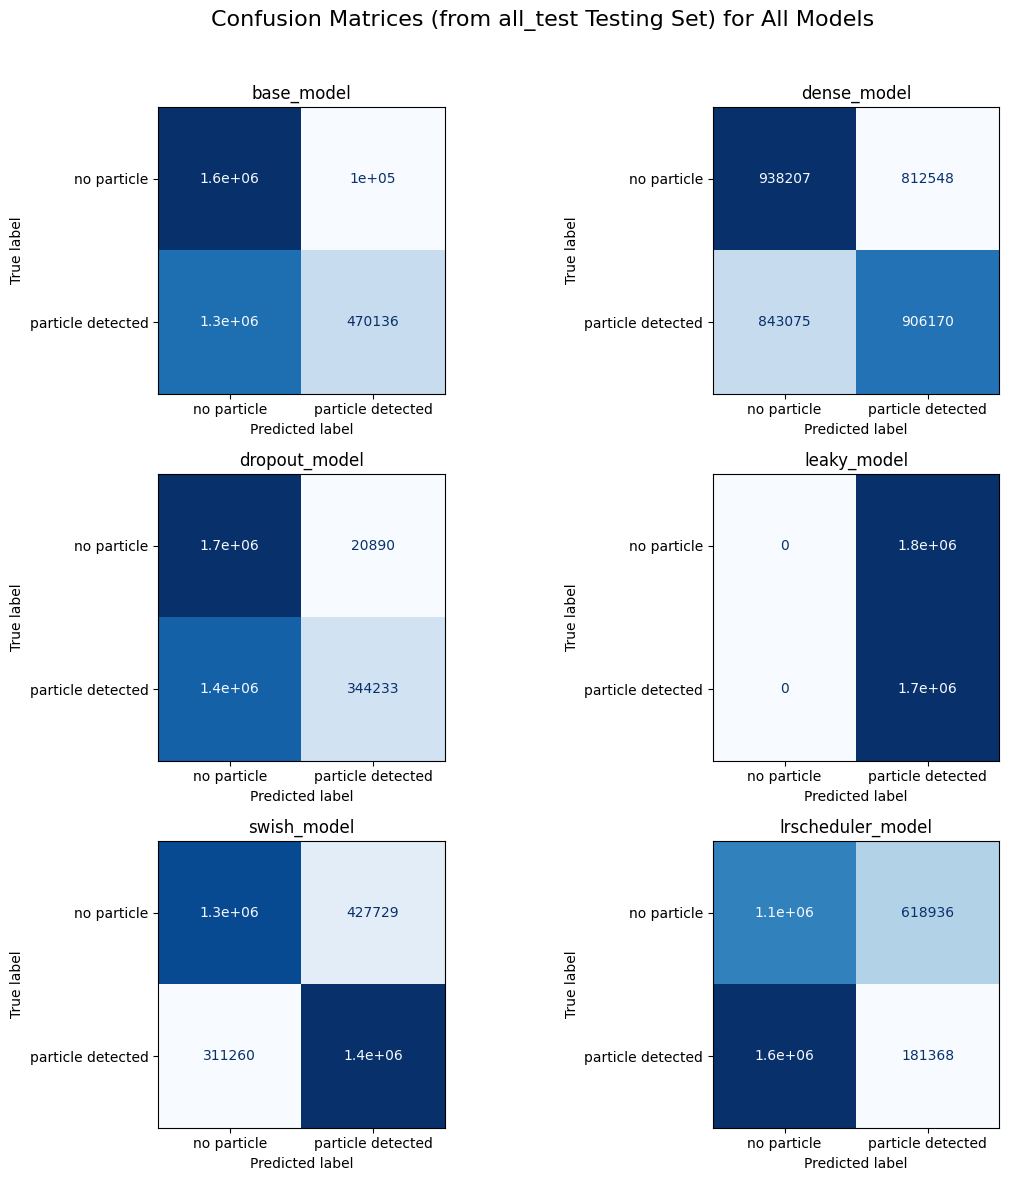
\includegraphics[width=1.0\textwidth]{figures/confusion_matrices_all_test.png}
	\caption{Confusion matrices showing classification results from the independent test set (\texttt{all\_test}) for all models. True labels are on the vertical axis and predicted labels on the horizontal axis. Each cell indicates the number of instances classified into each category.}
	\label{fig:test_confusion_matrices}
\end{figure}

\subsubsection{Overall Metrics}

With accuracy, macro-averaged precision, recall, and F1-score all near 79\%, the Swish model achieved the highest overall performance.

The LRScheduler model had low scores across all metrics, with accuracy and recall around 38\%, and precision and F1-score around 32--33\%.

The Dropout model achieved relatively high precision (0.7473), but its recall and F1-score were substantially lower. The Base model performed surprisingly well, with balanced metrics not far behind those of the Swish model.

The Leaky model exhibited highly inconsistent results due to its extreme bias toward predicting the \texttt{particle detected} class.

Macro-averaged metrics are reported here and are nearly identical to weighted averages due to the class balance in the test set. A visual summary of model performance on the test set is provided in Figure~\ref{fig:test_metrics_bar}.

\begin{table}[!htbp]
    \centering
    \caption{Overall Metrics by Model on the Independent Test Set}
    \begin{tabular}{lcccc}
    \arrayrulecolor{black}
    \toprule
    \textbf{Model} & \textbf{Accuracy} & \textbf{\makecell{Macro\\Precision}} & \textbf{\makecell{Macro\\Recall}} & \textbf{\makecell{Macro\\F1}} \\
    \midrule
    \arrayrulecolor{lightgray}
    Base & 0.6055 & 0.6927 & 0.6054 & 0.5550 \\ \hline
    Dense & 0.5270 & 0.5270 & 0.5270 & 0.5269 \\ \hline
    Dropout & 0.5926 & 0.7473 & 0.5924 & 0.5169 \\ \hline
    Leaky & 0.4998 & 0.2499 & 0.5000 & 0.3332 \\ \hline
    Swish & 0.7889 & 0.7901 & 0.7889 & 0.7886 \\ \hline
    LRScheduler & 0.3752 & 0.3229 & 0.3751 & 0.3255 \\
    \arrayrulecolor{black}
    \bottomrule
    \end{tabular}
    \caption*{\small\textit{Note: Macro and weighted metrics are nearly identical due to class balance. Only macro-averaged metrics are reported for brevity.}}
    \label{table:test_metrics_overall}
\end{table}

\begin{figure}[!htbp]
    \centering
    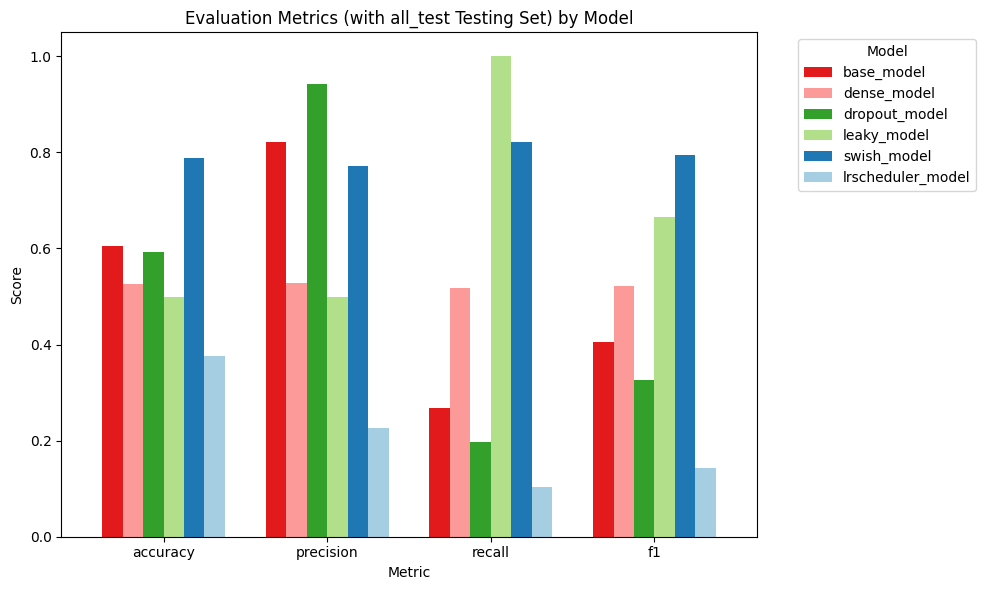
\includegraphics[width=0.80\textwidth]{figures/evaluation_metrics_all_test.png}
    \caption{Bar chart of independent test set performance metrics (accuracy, precision, recall, F1-score) for each model. Values reflect macro-averaged scores.}
    \label{fig:test_metrics_bar}
\end{figure}

\subsubsection{Per-Class Metrics}

As shown in Table~\ref{table:test_metrics_by_class}, the models varied drastically in their performance by class, and no single pattern applied across all models.

For the \texttt{no particle} class, the Swish model achieved the highest precision (0.8095), while the Dropout and Base models had the highest recall (0.9881 and 0.9420, respectively). The highest F1-score for this class was also achieved by the Swish model (0.7817), followed closely by the Dropout (0.7081) and Base (0.7049) models. The Leaky model predicted all observations as the \texttt{particle detected} class, resulting in zero true positives and zero predicted positives for the \texttt{no particle} class—leading to precision, recall, and F1-score values of 0.

For the \texttt{particle detected} class, the Dropout model achieved the highest precision (0.9428), while the Leaky and Swish models had the highest recall (1.0000 and 0.8221, respectively). The Leaky model's prediction of all events as \texttt{particle detected} yielded perfect recall but very low precision. The Swish model achieved the highest F1-score (0.7956) for this class.

Overall, the Swish model had the most balanced performance. The metrics precision, recall, and F1-score all exceeded 0.75 for both classes.

\begin{table}[H]
    \centering
    \caption{Per-Class Classification Metrics for Each Model on the Independent Test Set}
    \begin{tabular}{llrrrr}
    \arrayrulecolor{black}
    \toprule
    \textbf{Model} & \textbf{Class} & \textbf{Precision} & \textbf{Recall} & \textbf{F1-score} & \textbf{Support} \\
    \midrule
    Base & no particle         & 0.5632 & 0.9420 & 0.7049 & 1{,}750{,}755 \\
    & particle detected   & 0.8223 & 0.2688 & 0.4051 & 1{,}749{,}245 \\
    \midrule
    Dense & no particle         & 0.5267 & 0.5359 & 0.5313 & 1{,}750{,}755 \\
    & particle detected   & 0.5272 & 0.5180 & 0.5226 & 1{,}749{,}245 \\
    \midrule
    Dropout & no particle         & 0.5518 & 0.9881 & 0.7081 & 1{,}750{,}755 \\
    & particle detected   & 0.9428 & 0.1968 & 0.3256 & 1{,}749{,}245 \\
    \midrule
    Leaky & no particle         & 0.0000 & 0.0000 & 0.0000 & 1{,}750{,}755 \\
    & particle detected   & 0.4998 & 1.0000 & 0.6665 & 1{,}749{,}245 \\
    \midrule
    Swish & no particle         & 0.8095 & 0.7557 & 0.7817 & 1{,}750{,}755 \\
    & particle detected   & 0.7707 & 0.8221 & 0.7956 & 1{,}749{,}245 \\
    \midrule
    LRScheduler & no particle         & 0.4192 & 0.6465 & 0.5086 & 1{,}750{,}755 \\
    & particle detected   & 0.2266 & 0.1037 & 0.1423 & 1{,}749{,}245 \\
    \bottomrule
    \end{tabular}
    \label{table:test_metrics_by_class}
\end{table}

\section{Conclusion}

Among the six neural network models, the Swish model (using the SiLU activation function) showed the strongest and most generalizable performance. On the validation set, it came in just behind the Dropout model in accuracy (88.44\% vs. 88.46\%), but made predictions slightly faster and had comparable macro-averaged precision, recall, and F1-score. Both the Swish and Dropout models---differing only in activation function (SiLU vs. GELU)---exhibited a consistent class-specific pattern: higher recall than precision for the \texttt{particle detected} class and the reverse for the \texttt{no particle} class. This suggests they leaned toward identifying events as signal, capturing more true positives at the expense of increased false positives.

Due to the randomness introduced by dropout layers, training results for models that used dropout (the Dropout, Leaky, Swish, and LRScheduler models) may vary slightly between training runs. This variability is worth keeping in mind, as it can lead to small differences in performance metrics or convergence behavior, even with a fixed seed.

On the independent \texttt{all\_test} set, the Swish model was the only one that held up well, achieving 78.89\% accuracy---over 18 points higher than any other model. In contrast, other models struggled, often misclassifying large portions of the test data. The Leaky and LRScheduler models in particular showed how small changes, like switching activation functions or learning rate schedules, can make a big difference in how models generalize to new data.

Overall, this comparison highlights how architectural choices like dropout, activation function, optimizer can impact model behavior, especially when evaluated on unseen data. Future work could explore additional architectures, activation functions, and regularization techniques, as well as testing performance across diverse datasets to better understand model robustness.

\end{document}
